% Preamble
\documentclass[handout]{beamer}
\usepackage[utf8]{inputenc}
\usepackage{german}
\usepackage{ngerman}
\usepackage{tikz}
\usepackage{pgfplots}
\usepackage{eurosym}
\usepackage{amsmath}
\usepackage{lipsum}
\usepackage{tabularx}

\title[TSP]
{Travelling Salesman Problem}
\subtitle{Exakte Lösungen}
\author
{Axel Christ}
\institute{DHBW Karlsruhe}
\subject{Theorieseminar Informatik}

\newcommand{\centeredimage}[2]{
  \begin{figure}
    \centering
    \includegraphics[width=\linewidth,height=150px,keepaspectratio]{#1}
    \caption{#2}
  \end{figure}
}

\newcommand{\imageslide}[2]{
  \begin{frame}
    \centeredimage{#1}{#2}
  \end{frame}
}

\newcommand{\fullscreenimage}[1]{
  { % all template changes are local to this group.
    \setbeamertemplate{navigation symbols}{}
    \begin{frame}[plain]
        \begin{tikzpicture}[remember picture,overlay]
            \node[at=(current page.center)] {
                \includegraphics[width=\paperwidth,height=\paperheight,keepaspectratio]{#1}
            };
        \end{tikzpicture}
     \end{frame}
  }
}

\newcommand{\sloganslide}[2]{
  \begin{frame}
    \begin{center}
      \Huge #1
      \ifx&#2&%
        \huge #2
      \fi
    \end{center}
  \end{frame}
}

\AtBeginSection[]
{
  \begin{frame}
    \frametitle{Table of Contents}
    \tableofcontents[currentsection]
  \end{frame}
}

\begin{document}
  \fullscreenimage{buyonline.jpeg} % Wir kaufen einen neuen Laptop online

  \fullscreenimage{postbote.jpg} % Versand natürlich mit der Post, aber

  \sloganslide{Wie sieht eigentlich die Tour des Postboten aus?}

  \fullscreenimage{deutschland.png} % Planung einer Tour zu den Kunden

  \imageslide{deutschland_solved.jpg}{Gelöst 2001: 15,112 Städte in Deutschland}

  \imageslide{schweden_solved.jpg}{Gelöst 2004: 24,978 Städte in Schweden}

  \sloganslide{Und doch NP-Vollständig?}

  \frame{\titlepage}

  \begin{frame}
    \frametitle{Anwendungsbereiche}

    \begin{itemize}
      \item Tourplanung 
      \item Logistik
      \item Mikrochips
      \item Genom-Sequenzierung
    \end{itemize}
  \end{frame}

  \section{Definition}
  \begin{frame}
    \frametitle{Definition}
    \begin{center}
      Ein Handlungsreisender muss mehrere Städte besuchen. Dabei soll die
      Strecke, um alle Städte zu besuchen, möglichst kurz sein.
    \end{center}
  \end{frame}

  \begin{frame}
    \frametitle{Definition}
    Es gibt $N$ Städte.
    \pause
    \\~\\

    Zwischen zwei Städten $i$ und $j$ gibt es jeweils eine Kante $c_{ij}$.
    Sollte einmal keine Kante bestehen, so wird eine Kante mit großer Länge
    automatisch eingefügt. Repräsentiert wird das Problem als ein Graph.
    \pause
    \\~\\

    Zu jeder Kante (Verbindung zwischen zwei Städten) gibt es eine Länge $c_{i,j} \geq 0$
    \pause
    \\~\\

    Gesucht ist ein Hamiltonkreis, der jeden Knoten (jede Stadt) genau einmal enthält.
    Dabei soll der Umfang des Hamiltonkreises minimiert werden, eine möglichst kurze Tour
    soll gefunden werden.
  \end{frame}

  \begin{frame}
    \frametitle{TSP-Klassifikationen}
    \begin{itemize}[<+->]
      \item \textbf{Symmetrisches TSP}
        \linebreak
        Ungerichteter Graph
        $$c_{ij} = c_{ji}$$
        Hin- und Rückweg zwischen zwei Knotenpunkten stets gleich
      \item \textbf{Asymmetrisches TSP}
        \linebreak
        Gerichteter Graph
        Hin- und Rückweg zwischen zwei Knotenpunkten muss nicht gleich sein
      \item \textbf{Metrisches TSP}
        \linebreak
        Erfüllen der Dreiecksungleichung
        $$c_{ij} \le c_{ik} + c_{kj}$$
        Verbindung von $i$ nach $j$ nie länger als über dritten Knoten $k$
    \end{itemize}
  \end{frame}

  \begin{frame}
    \frametitle{Nicht-metrisches TSP}
    Ein TSP-Problem kann auch nicht-metrisch sein, wenn Umrüstzeiten
    berücksichtigt werden müssen.
    \pause
    \linebreak
    Beispiel: Drei Trucks sollen an verschiedenen Stationen Gegenstände
    abliefern und aufnehmen:
    \begin{figure}
      \centering
      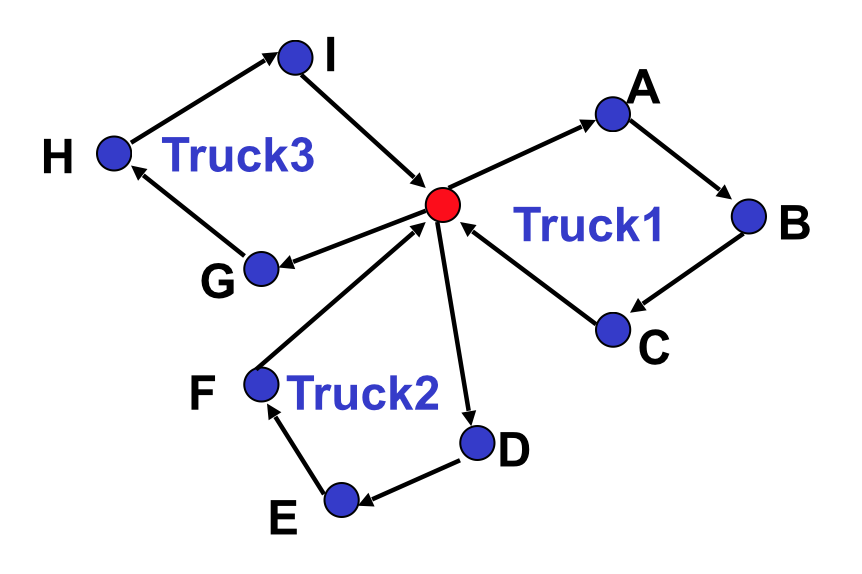
\includegraphics[width=\linewidth,height=150px,keepaspectratio]{truck_problem.png}
      \caption{Truck Problem}
    \end{figure}
  \end{frame}

  \section{Komplexität}
  \begin{frame}
    \frametitle{Komplexitätsbetrachtung}
    Bei einem symmetrischen TSP gibt es $\frac{(n-1)!}{2}$ mögliche Routen,
    bei einem asymmetrischen $(n-1)!$ mögliche!

    \newcount\mycount

    \begin{figure}
      \centering
      \begin{tikzpicture}[transform shape,scale=0.4]
        %the multiplication with floats is not possible. Thus I split the loop in two.
        \foreach \number in {1,...,8}{
            % Computer angle:
              \mycount=\number
              \advance\mycount by -1
        \multiply\mycount by 45
              \advance\mycount by 0
            \node[draw,circle,inner sep=0.25cm] (N-\number) at (\the\mycount:5.4cm) {};
          }
        \foreach \number in {9,...,16}{
            % Computer angle:
              \mycount=\number
              \advance\mycount by -1
        \multiply\mycount by 45
              \advance\mycount by 22.5
            \node[draw,circle,inner sep=0.25cm] (N-\number) at (\the\mycount:5.4cm) {};
          }
        \foreach \number in {1,...,15}{
              \mycount=\number
              \advance\mycount by 1
        \foreach \numbera in {\the\mycount,...,16}{
          \path (N-\number) edge[->,bend right=3] (N-\numbera)  edge[<-,bend
            left=3] (N-\numbera);
        }
      }
      \end{tikzpicture}
      \caption{Anzahl mögliche Verbindungen bei $n=16$}
    \end{figure}
  \end{frame}

  \begin{frame}
    \frametitle{Verbindungen}

    Woher bekommt man die Informationen über Verbindungslängen?
    \pause
    \vspace{2em}

    Dijkstra-Algorithmus benötigt pro Strecke ca $10s$ (Trotz Einschränkungen)

    \pause
    \vspace{1em}

    \textbf{Beispiel}: Bei 1000 Städten: \\~\\
    $1000 \cdot 1000 = 1 000 000$ mögliche Verbindungen!
    $\rightarrow 1 000 000 \cdot 10s = 10 000 000s \approx 116 Tage$,
    deshalb in Praxis oft 1.3 * Luftlinie

    \vspace{1em}
    Laufzeit Dijkstra: $\mathcal O(n \cdot \log n + m)$ \textit{(optimiert)}
    \\~\\
    $n$ Anzahl der Knoten, $m$ Anzahl der Kanten
  \end{frame}

  \section{Mathematische Betrachtung}

  \begin{frame}
    \frametitle{Mathematische Betrachtung}
    \begin{itemize}
      \item Knotenmenge $V$
      \item Pro Kante ein Bit $x$:
      \begin{itemize}
        \item $x=1 \rightarrow$ Kante ist in Tour enthalten
        \item $x=0 \rightarrow$ Kante ist nicht in Tour enthalten 
      \end{itemize}
    \end{itemize}
    \textbf{Aufgabe ist:}
    $$min\sum_{i \in V} \sum_{j \in V \backslash i} c_{i,j}x_{i,j}$$
  \end{frame}

  \sloganslide{Ist jede somit definierte Tour valide?}

  \fullscreenimage{nodes.png}

  \fullscreenimage{invalid_tour.png}

  \begin{frame}
    \frametitle{Randbedingungen}
    \begin{Large}
      \begin{center}
        Jeder Knoten muss exakt 2 Verbindungen haben!
      \end{center}

      \pause
      \textbf{Deshalb:}
      $$\sum_{j \in V \backslash i}x_{i,j} = 2$$
    \end{Large}
  \end{frame}

  \sloganslide{Sind somit alle Touren valide?}

  \fullscreenimage{kurzkreiszyklen.png}

  \begin{frame}
    \frametitle{Randbedingungen}
    \begin{Large}
      \begin{center}
        Alle Knoten sollen in einer Tour miteinander verbunden sein,
        keine \textit{Kurzkreiszyklen} sollen entstehen!
      \end{center}

      \pause
      \textbf{Deshalb:}
      $$\sum_{i \in S, j \notin S}x_{i,j} \geq 2$$
    \end{Large}
  \end{frame}

  \begin{frame}
    \frametitle{Mathematische Betrachtung}
    \begin{itemize}
      \item Knotenmenge $V$
      \item Pro Kante ein Bit $x$:
      \begin{itemize}
        \item $x=1 \rightarrow$ Kante ist in Tour enthalten
        \item $x=0 \rightarrow$ Kante ist nicht in Tour enthalten 
      \end{itemize}
      \item
        Pro Knoten (Stadt) genau zwei Kanten
        $$\sum_{j \in V \backslash i}x_{i,j} = 2$$
      \item
        Keine Kurzkreiszyklen
        $$\sum_{i \in S, j \notin S}x_{i,j} \geq 2$$
    \end{itemize}
    \pause
    \textbf{Aufgabe ist:}
    $$min\sum_{i \in V} \sum_{j \in V \backslash i} c_{i,j}x_{i,j}$$
  \end{frame}

  \section{Exakte Lösungen}

  \begin{frame}
    \frametitle{Lösung durch Permutation}

    \begin{enumerate}[<+->]
      \item Permutation durch alle möglichen Touren
      \item Für kleine $n$ noch machbar
      \item Jedoch: $n$ steigt schnell drastisch an (Fakultät)
    \end{enumerate}

    \pause

    \begin{figure}
      \centering
      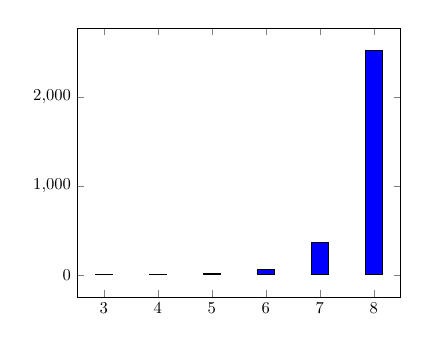
\begin{tikzpicture}[scale=0.6]
        \begin{axis}[
            symbolic x coords={3, 4, 5, 6, 7, 8},
            xtick=data
          ]
            \addplot[ybar,fill=blue] coordinates {
                (3, 1)
                (4, 3)
                (5, 12)
                (6, 60)
                (7, 360)
                (8, 2520)
            };
        \end{axis}
      \end{tikzpicture}
      \caption{Anzahl Touren in Abhängigkeit $n$ bei symmetrischem TSP}
    \end{figure}
  \end{frame}

  \subsection{Lineare Programmierung}
  \begin{frame}
    \frametitle{Problemstellung}

    Eine Möbelfirma produziert zwei Arten von Sofas: Ein Standard-
    und ein Sondermodell.
    \pause
    \\~\\

    Die Produktion eines Standardmodells benötigt zwei Stunden, die
    eines Sondermodells drei.
    \pause
    \\~\\

    Drei Arbeiter arbeiten jew. 8 Stunden am Tag
    \pause
    \\~\\

    Der maximale tägliche Bedarf an Standardsofas ist 6, bei
    Sondersofas 8.
    \pause
    \\~\\

    Ein Standardsofa bringt 500\euro, ein Sondermodell 300\euro.
    \pause
    \\~\\

    \textbf{Wie kann der Profit der Möbelfirma maximiert werden?}
  \end{frame}

  \begin{frame}
    \frametitle{Datenanalyse}

    \textbf{Was sind die Entscheidungsvariablen?}
    \linebreak
    \pause
    Anzahl der Standardsofas ($x$) und Anzahl der Sondersofas ($y$) die pro
    Tag produziert werden sollen.
    \pause
    \\~\\

    \textbf{Was sind die Randbedingungen?}
    \pause
    \begin{itemize}[<+->]
      \item Verfügbare Arbeitskapazität pro Tag: $3 \cdot 8 = 24$
      \item Maximale Nachfrage pro Tag
        \begin{itemize}
          \item Standardsofas: 6
          \item Sondersofas: 8 
        \end{itemize}
      \item Zeitverbrauch pro Einheit
        \begin{itemize}
          \item Standardsofa: 2h
          \item Sondersofa: 3h 
        \end{itemize}
    \end{itemize}
  \end{frame}

  \begin{frame}
    \frametitle{Mathematische Repräsentation}

    \textbf{Zielfunktion}
    $$f(x) = 500x \cdot 300y $$
    \pause

    \textbf{Nachfrage}
    $$x \leq 6$$
    $$y \leq 8$$
    \pause

    \textbf{Max. Arbeitskapazität}
    $$2x + 3y \leq 24$$
    \pause

    \textbf{Entscheidungsvariablen müssen nichtnegativ sein}
    $$x, y \geq 0$$
  \end{frame}

  \begin{frame}
    \frametitle{Graphische Repräsentation}
    \begin{columns}[onlytextwidth]
      \begin{column}{0.4\textwidth}
        \begin{itemize}[<+->]
          \item Anfänglich: Alle Werte möglich
          \item Dann: Beschränken durch Constraints
          \item Zusätzlich: Anzeige der Fitnessfunktion
        \end{itemize}
      \end{column}
      \begin{column}{0.6\textwidth}
        \begin{figure}
          \centering
          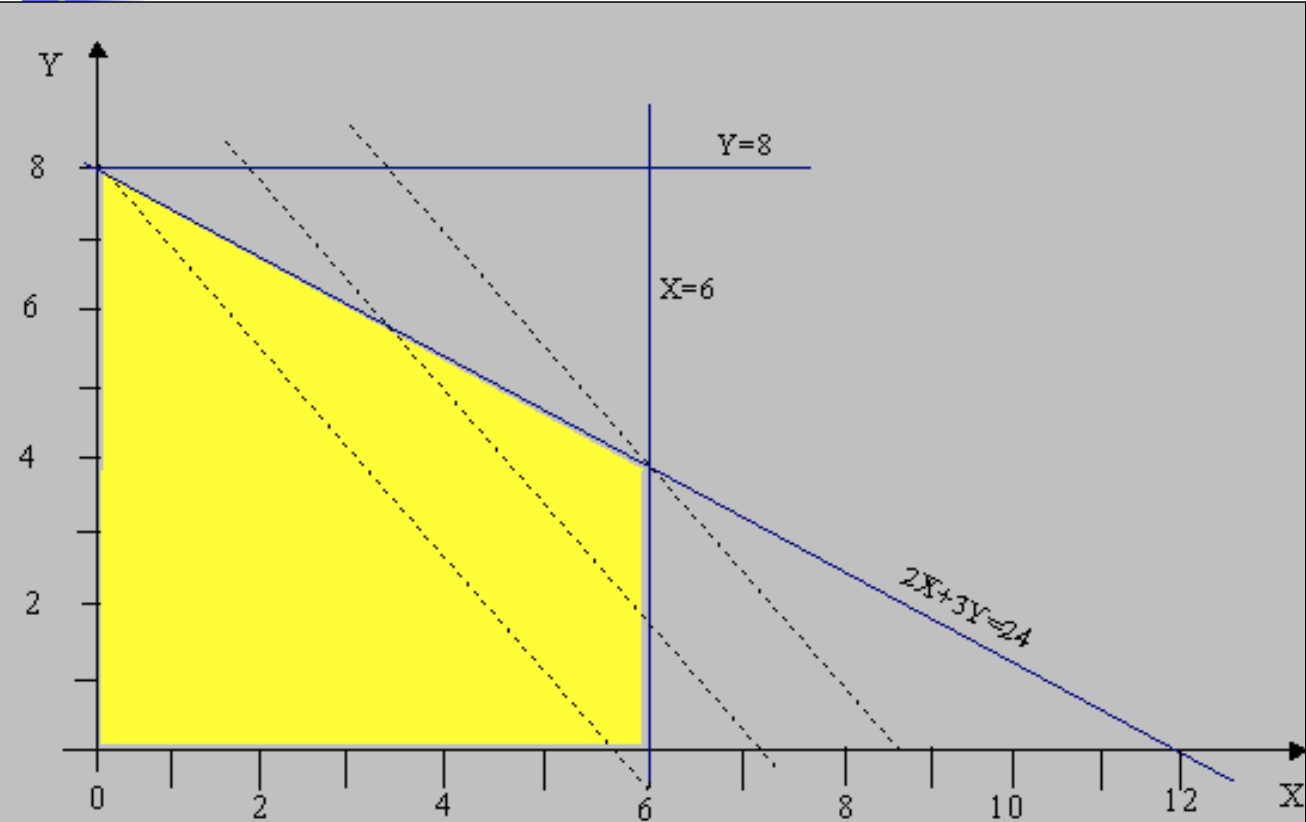
\includegraphics[width=\linewidth,height=150px,keepaspectratio]{optimization_graphic.png}
        \end{figure}
      \end{column}
    \end{columns}
  \end{frame}

  \begin{frame}
    \frametitle{Problem der Lösung}
    \begin{columns}[onlytextwidth]
      \begin{column}{0.4\textwidth}
        \begin{itemize}[<+->]
          \item Lösung liegt immer in den Eckbereichen der zulässigen Lösungen
          \item Lösung liegt oft im kontinuierlichen
          \item \textbf{Jedoch:} Für Sofaproblem sollten nur ganzzahlige Lösungen akzeptiert werden!
        \end{itemize}

        \pause

        \textbf{$\rightarrow$ Andere Lösungsmethoden benötigt!}
      \end{column}
      \begin{column}{0.6\textwidth}
        \begin{figure}
          \centering
          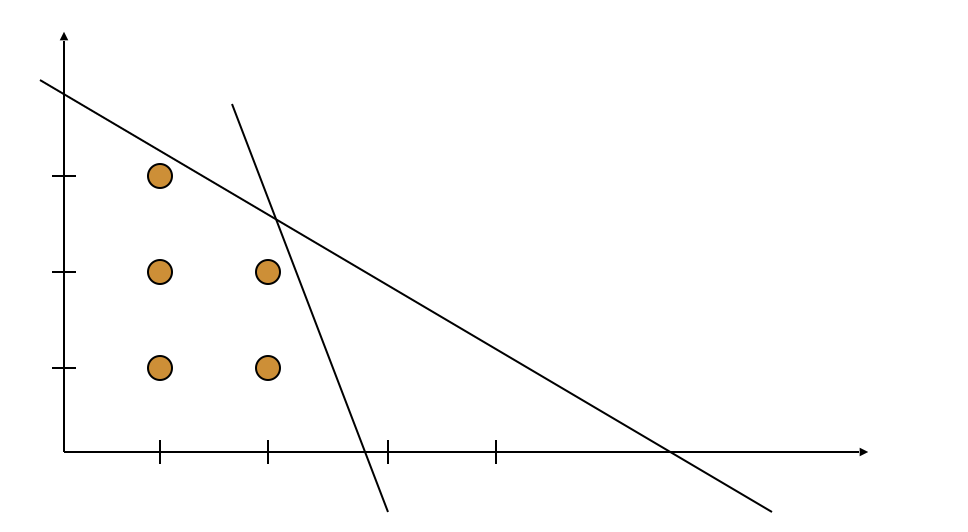
\includegraphics[width=\linewidth,height=150px,keepaspectratio]{mlp_solutions.png}
        \end{figure}
      \end{column}
    \end{columns}
  \end{frame}

  \subsubsection{Branch and Bound}
  \begin{frame}
    \frametitle{Branch and Bound}

    Lösungsmethode von Ganzzahligen Problemen
    \begin{enumerate}[<+->]
      \item Lineare Relaxierung des Problems
      \item Verzweigen
      \item Begrenzen
      \item Optimalitätstest
    \end{enumerate}
  \end{frame}

  \begin{frame}
    \frametitle{Branch and Bound}
    \textbf{Beispiel}
    $$z = x + 4 * y$$

    Constraints:
    \begin{itemize}
      \item $5x + 8y \leq 40$
      \item $-2x + 3y \leq 9$
      \item $x, y \geq 0$ 
    \end{itemize}

    \pause
    \vspace{1em}

    \textit{Lösung ohne ganzzahlige Beschränkung}
    $$x = 1\frac{17}{31}, y = 4\frac{1}{31}, z = 17\frac{21}{31}$$
  \end{frame}

  \begin{frame}
    \frametitle{Grafische Visualisierung}
    \begin{figure}
      \centering
      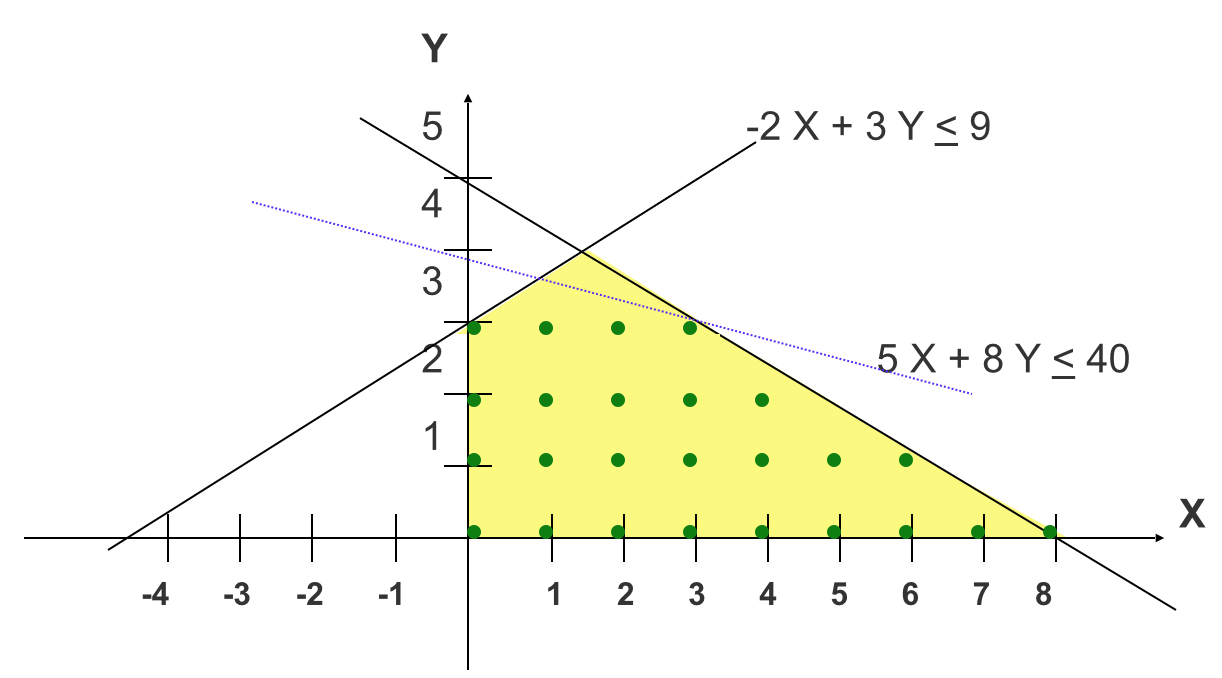
\includegraphics[width=\linewidth,height=150px,keepaspectratio]{example_graphical_representation.png}
      \caption{Mögliche Lösungen und Constraints des Problems}
    \end{figure}
  \end{frame}

  \begin{frame}
    \frametitle{Grafische Visualisierung}
    \begin{figure}
      \centering
      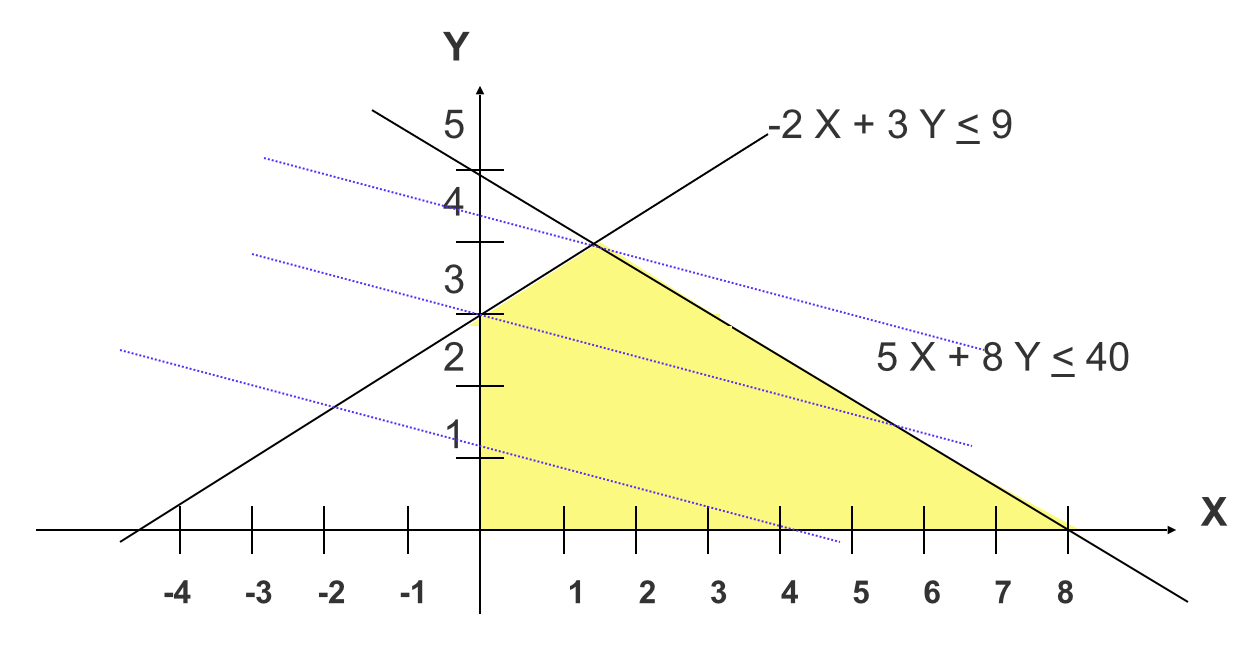
\includegraphics[width=\linewidth,height=150px,keepaspectratio]{example_noninteger_solution.png}
      \caption{Lösung nach linearer Relaxierung}
    \end{figure}
    $$x = 1\frac{17}{31}, y = 4\frac{1}{31}, z = 17\frac{21}{31}$$
  \end{frame}

  \foreach \x in {1,2,3,4,5,6,7,8,9,10,11,12}
  {
    \imageslide{branch_and_bound\x.png}{Branch and Bound \x}
  }

  \subsubsection{Cutting Planes}
  \begin{frame}
    \frametitle{Cutting Planes}

    \begin{itemize}
      \item Andere Methode der Linearen Programmierung
      \item Startpunkt ebenfalls relaxierte Lösung
      \item Unterschied: Schnittebenen, um Lösungsraum einzuschränken
      \item Schnittebenen sind im Allgemeinen weitere Constraint-Ungleichungen
    \end{itemize}
  \end{frame}

  \foreach \x in {1,2}
  {
    \imageslide{schnittebenen_\x.png}{Schnittebenen Veranschaulichung \x}
  }

  \begin{frame}
    \frametitle{Anforderungen an Schnittebenen}

    \begin{itemize}
      \item Keine mögliche Lösung darf abgeschnitten werden
      \item Die letzte, nichtganzzahlige Lösung soll abgeschnitten werden 
      \item $2^n$ Schnittebenen lösen Problem, jedoch werden typischerweise nur
      $n$ verletzte cuts generiert, damit alle exponentiell viele Schnittebenen erfüllt sind
    \end{itemize}

    \pause
    \textbf{Jedoch:} Lösung nicht immer ganzzahlig!
    \pause
    \\~\\

    $\rightarrow$ \textbf{Deshalb:} Kombination beider Ansätze zu \textit{Branch and Cut}
  \end{frame}

  \section{Concorde TSP Solver}
  \begin{frame}
    \frametitle{Vorgehensweise}

    Ähnlich wie bei Branch and Bound, jedoch wird vor Verzweigung
    versucht, mit Schnittebenen den Lösungsraum einzugrenzen.

    \pause
    \vspace{1em}

    Nach Eingrenzung durch Schnittebenen: \\~\\
    \textit{Ist Lösung ganzzahlig?}

    \pause
    \vspace{1em}

    \textbf{Falls ja:} Lösung optimal, Abbruch
    \pause
    \textbf{Falls nein:} Aufsplitten wie bei Branch and Bound, rekursive Anwendung
  \end{frame}

  \begin{frame}
    \frametitle{Programme in der Praxis}
    Anwendung in der Praxis mit Programm \textit{Concorde}
  \end{frame}

  \begin{frame}[t]{Concorde}
    \begin{table}\scriptsize
    \begin{tabularx}{\textwidth}{l c c | l c c}
      \textbf{Name} & \textbf{Time} & \textbf{Search Nodes} & \textbf{Name} & \textbf{Time} & \textbf{Search Nodes} \\
  burma14&0.02&1& ulysses16&0.12&1 \\
  gr17&0.04&1&  gr21&0.01&1 \\
  ulysses22&0.29&1& gr24&0.02&1 \\
  fri26&0.03&1& bayg29&0.05&1 \\
  bays29&0.04&1&  dantzig42&0.09&1 \\
  swiss42&0.05&1& att48&0.22&1 \\
  gr48&0.18&1&  hk48&0.08&1 \\
  eil51&0.12&1& berlin52&0.13&1 \\
  brazil58&0.24&1&  st70&0.20&1 \\
  eil76&0.11&1& pr76&0.60&1 \\
  gr96&0.84&1&  rat99&0.40&1 \\
  kroA100&0.31&1& kroB100&0.58&1 \\
  kroC100&0.30&1& kroD100&0.33&1 \\
  kroE100&0.75&1& rd100&0.22&1 \\
  eil101&0.24&1&  lin105&0.22&1 \\
  pr107&0.37&1& gr120&0.48&1 \\
  pr124&1.04&1& bier127&0.53&1 \\
  ch130&0.65&1& pr136&1.12&1 \\
  gr137&2.18&1& pr144&1.01&1 \\
  ch150&0.91&1& kroA150&1.47&1 \\
  kroB150&2.50&3& pr152&2.98&1 \\
  u159&0.42&1&  si175&5.75&3 \\
  \end{tabularx}
  \end{table}
  \end{frame}


  \begin{frame}[t]{Concorde}
    \begin{table}\scriptsize
    \begin{tabularx}{\textwidth}{l c c | l c c}
      \textbf{Name} & \textbf{Time} & \textbf{Search Nodes} & \textbf{Name} & \textbf{Time} & \textbf{Search Nodes} \\
  brg180&0.26&1&  rat195&6.25&3 \\
  d198&3.83&3&  kroA200&2.24&1 \\
  kroB200&1.06&1& gr202&2.90&1 \\
  ts225&7.04&1& tsp225&5.18&1 \\
  pr226&1.06&1& gr229&12.40&7 \\
  gil262&3.61&3&  pr264&1.05&1 \\
  a280&2.48&1&  pr299&5.33&1 \\
  lin318&2.78&1&  rd400&25.72&9 \\
  fl417&23.48&3&  gr431&31.94&9 \\
  pr439&73.62&15& pcb442&9.44&9 \\
  d493&43.13&5& att532&32.24&5 \\
  ali535&9.50&1&  si535&21.73&3 \\
  pa561&52.06&7&  u574&22.99&3 \\
  rat575&70.30&17&  p654&8.57&1 \\
  d657&83.04&13&  gr666&31.31&7 \\
  u724&73.78&15&  rat783&16.79&1 \\
  dsj1000&153.16&13&  pr1002&9.92&1 \\
  si1032&107.19&1&  u1060&141.12&13 \\
  vm1084&234.66&13& pcb1173&168.11&13 \\
  rl1304&103.01&1&  nrw1379&108.12&7 \\
  u1432&35.90&1&  d1655&69.08&3 \\
  pr2392&35.04&1
    \end{tabularx}
  \end{table}
  \end{frame}

  \begin{frame}
    \frametitle{Fazit - Trotz allem NP-Schweres Problem}

    \Large Euklidische TSP-Probleme mit zufälligen Knoten oder typischen TSP-Anwendungen
    können sehr schnell gelöst werden

    \pause
    \vspace{2em}

    \Large Bei Übersetzung eines anderen schwierigen Optimierungsproblem in TSP jedoch
    sehr schwer zu lösen!
  \end{frame}

  \sloganslide{Vielen Dank für eure Aufmerksamkeit!}

\end{document}